\chapter{ND4J}
\label{chap:java_nd4j}

\section{ND4J介绍}

Nd4j是一个基于JVM的,接口和numpy接近的张量运算库。目前流行的数据分析框架,大多是基于Python或MatLab开发的,很难移植到JVM运行环境。
虽然有Colt这样的Java类库,但它对商业不友好。
\vspace{0.5cm}\noindent

\emph{ND4J主要特点:}(摘自官网)
\begin{itemize}
\item[1.] 多用途多维数组对象
\item[2.] 支持多平台扩展,包括GPU
\item[3.] 提供线性代数和信号处理功能
\end{itemize}

\noindent
使用ND4J创建多维向量和矩阵非常容易,用起来和numpy非常类似,甚至还提供了ND4S这种更加接近numpy的类库。

\noindent \ \\
\emph{创建2X2的NDArray:}
\begin{lstlisting}[language=Java]
INDArray arr1 = Nd4j.create(new float[]{1,2,3,4},new int[]{2,2});
System.out.println(arr1);
\end{lstlisting}
输出:
[[1.0 ,3.0]
[2.0 ,4.0]
]

\section{使用ND4J}
在学习使用ND4J之前,有必要了解数组在内存中的组织方式。数组通常是一段连续的内存,但Java并不能保证整个维度是连续的,这也很容易证明:

\begin{lstlisting}[language=Java,caption={Java二维数组},label=code:part3_array_mem]
int[][] numbers = new int[2][];
int[] N1 = {1,2,3};
int[] N2 = {2,3,4};

numbers[0] = N1;
numbers[1] = N2;
\end{lstlisting}

\coderef{code:part3_array_mem},展示了N1和N2是2个不同的int[]对象,但无法确定数据在内存中的组织是否连续。Java这种分散的数据组织范式,非常不利于批量运算和GPU加速。
为了更有效率的使用数据,ND4J没采用Java的多维数组形式来表示张量(标量、向量、矩阵),而是在JVM之外申请的内存。
不仅有更好的性能,还可以结合更多的Native加速线性代数库,譬如BLAS。
\footnote{BLAS:Basic Linear Algebra Subprograms,目前最快的是Intel的MKL}

\begin{figure}[!htb]
\centerline{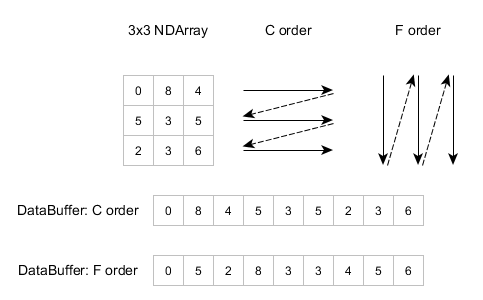
\includegraphics[width=.35\figwidth]{images/c_vs_f_order.png}}
\label{fig:part3_c_vs_f_order}
\caption{C序和F序}
\end{figure}

\noindent
\figref{fig:part3_c_vs_f_order}展示了这种不同。创建NDArray的时候,可以指定使用哪种方式。

\subsection{创建和更新}
与前面IntVector不同的是,NDArray的数据只有double或float类型,并且所有的NDArray共享相同的dtype。默认情况下,NDArray的数据都是float类型的。
创建NDArray有很多方式,ND4J还为全0和全1数组提供了便利接口:
\vspace{0.3cm}

\begin{lstlisting}[language=Java]
Nd4j.zeros(int...)
Nd4j.ones(int...)
\end{lstlisting}
\noindent
其中,int...是维度信息。

创建一般的NDArray则可以用章节一开始时提到的create()方法,传入两个数组作为数据组和维度即可。

另外,对于元素服从正态分布的NDArray,或是元素属于(0,1)区间的NDArray,ND4J都提供了相应的接口:
\begin{lstlisting}[language=Java]
Nd4j.rand(int,int);
Nd4j.randn(int,int);
\end{lstlisting}

在DL4J中,更新操作也很便利,利用putScalar和putRow方法,传入需要改变元素的位置与值,即可完成操作,
例如下面的代码,putScalar方法将矩阵下标为(1,3)的元素修改成100,putRow方法则将第一行
的所有元素重新设置成传入的INDArray中对应的元素,这样就完成了元素的更新。

\begin{lstlisting}[language=Java]
arr1.putScalar(1, 3, 100);
arr1.putRow(1,INDArray);
\end{lstlisting}

\subsection{切片操作}

对于NDArray,我们往往需要其中的一部分来进行操作,这就需要用切片操作来完成。
切片操作的代码如下图所示,我们传入一个或多个行数信息,就能获得对应行数的NDArray。
但是需要注意的是这两种方法只适用于二维矩阵。

\begin{lstlisting}[language=Java]
arr1.getRow(int);
arr1.getRows(int...);
\end{lstlisting}


但在日常使用中,我们对NDArray的切片要求往往更加复杂,仅仅使用上述的两个方法会比较困难。
例如我们对一个NDArray进行取前三行,前三列的操作时,仅仅用getRow和getRows方法就显得比较麻烦。
这时我们就需要用get方法进行操作:

\begin{lstlisting}[language=Java]
arr1.create(new float[]{1,2,3,4,5,6,7,8,9},new int[]{3,3});
INDArray arr2 = arr1.get(NDArrayIndex.interval(0,2), NDArrayIndex.interval(0,2));
System.out.println(arr2);
\end{lstlisting}

\noindent
输出结果为[[1.0,2.0] [4.0,5.0]],这就完成了对NDArray的切片操作。

\subsection{基本运算}

NDArray的基本运算包括张量操作和元素操作。其中张量操作包括加减乘除四则运算,
操作对NDArray中的所有元素进行,在调用时传入一个数即可,例如:

\begin{lstlisting}[language=Java]
doube myDouble = 1.0;
INDArray arr1 = Nd4j.create(new float[]{1,2},new int[]{1, 2}); 
NDArray arr2 = arr1.add(myDouble);
arr1.sub(myDouble);
arr1.mul(myDouble);
arr1.add(myDouble);
System.out.println(arr2);
\end{lstlisting}

\noindent
输出结果为[[2.0,3.0]]。


元素操作与张量操作类似,都是对NDArray中的元素进行运算操作,不同的是张量操作传入的是一个数,
所有元素执行同一个操作;而元素操作传入一个NDArray,每个元素与另一个NDArray中对应的元素进行
操作。因此,元素操作要求进行操作的两个矩阵形状一致。

\begin{lstlisting}[language=Java]
INDArray arr1 = Nd4j.create(new float[]{1,2},new int[]{1, 2});
INDArray arr2 = Nd4j.create(new float[]{2,3},new int[]{1, 2});
System.out.println(arr1.add(arr2));
\end{lstlisting}

\noindent
输出结果为[[3.0,5.0]]。


\section{线性回归示例}








